\documentclass[xcolor=table]{beamer}
\setbeamertemplate{footline}[frame number]

\mode<presentation> {
\usepackage[utf8]{inputenc}
\usepackage[T1]{fontenc}
\usepackage[style=authoryear, backend=biber]{biblatex}
\addbibresource{references.bib}
\usepackage{hyphenat}
\usepackage{textpos}
\fboxsep0pt

\usepackage{array,booktabs}% http://ctan.org/pkg/{array,booktabs}
\usetheme{default}
%\usetheme{AnnArbor}
%\usetheme{Antibes}
%\usetheme{Bergen}
%\usetheme{Berkeley}
%\usetheme{Berlin}
%\usetheme{Boadilla}
%\usetheme{CambridgeUS}
%\usetheme{Copenhagen}
%\usetheme{Darmstadt}
%\usetheme{Dresden}
%\usetheme{Frankfurt}
%\usetheme{Goettingen}
%\usetheme{Hannover}
%\usetheme{Ilmenau}
%\usetheme{JuanLesPins}
%\usetheme{Luebeck}
%\usetheme{Madrid}
% \usetheme{Malmoe}
%\usetheme{Marburg}
%\usetheme{Montpellier}
%\usetheme{PaloAlto}
%\usetheme{Pittsburgh}
%\usetheme{Rochester}
%\usetheme{Singapore}
%\usetheme{Szeged}
%\usetheme{Warsaw}

%\usecolortheme{albatross}
%\usecolortheme{beaver}
%\usecolortheme{beetle}
%\usecolortheme{crane}
% \usecolortheme{dolphin}
%\usecolortheme{dove}
%\usecolortheme{fly}
%\usecolortheme{lily}
%\usecolortheme{orchid}
%\usecolortheme{rose}
%\usecolortheme{seagull}
%\usecolortheme{seahorse}
%\usecolortheme{whale}
%\usecolortheme{wolverine}


% \definecolor{presentationColor}{rgb}{0.2274, 0.4039, 0.5490} 
% \usecolortheme[named=presentationColor]{structure}
\setbeamertemplate{frametitle continuation}[from second][(cont.)]
\setbeamertemplate{navigation symbols}{} % To remove the navigation symbols from the bottom of all slides uncomment this line
}
\usepackage{graphicx} % Allows including images
\usepackage{booktabs} % Allows the use of \toprule, \midrule and \bottomrule in tables
\usepackage{caption}
\usepackage{subcaption}
\usepackage{xcolor}
\usepackage{amsfonts}
\usepackage{svg}
\usepackage{animate}
\usepackage{tikz}
\usepackage[customcolors]{hf-tikz}
\usepackage{listings}
\usepackage{xcolor}  % opcjonalnie, aby dodać kolory

\lstset{
  language=Python,          % Język programowania, np. Python, C, Java
  basicstyle=\ttfamily\footnotesize,  % Ustawienia wyglądu tekstu
  keywordstyle=\color{blue},          % Kolor dla słów kluczowych
  commentstyle=\color{gray},          % Kolor dla komentarzy
  stringstyle=\color{red},            % Kolor dla stringów
  showstringspaces=false,             % Nie pokazuj spacji w stringach
  breaklines=true,                    % Łam linie, jeśli są zbyt długie
}

\usetikzlibrary{arrows,shapes,snakes,positioning,fit,backgrounds,mindmap}

\tikzset{
    >=stealth',
    node/.style={
           rectangle,
           rounded corners,
           draw=black!80, very thick,
           text centered,
           inner sep=5pt
    },
    pil/.style={
           ->,
           thick,
           shorten <=2pt,
           shorten >=2pt}
}
\renewcommand*{\bibfont}{\scriptsize} 

%% \title[CUDA by examples: delay and sum]{CUDA by examples: delay and sum}
\title[CUDA streams and processing frameworks]{CUDA streams and processing frameworks} 
\author[P. Jarosik et al]{Piotr Jarosik, Marcin Lewandowski, Billy Yiu}
\titlegraphic{

}
\institute[IPPT PAN] 
{
\vspace{5mm}
GPU Short Course, IEEE UFFC-JS 2024
\medskip
}
\date{} 

\begin{document}

\begin{frame}
\titlepage
\end{frame}

\newcommand{\outline}{
\begin{frame}[allowframebreaks]{Agenda}
\frametitle{Agenda}
\tableofcontents 
\end{frame}
}
\newcommand{\references} {
\begin{frame}[allowframebreaks]{References}
\frametitle{References}
    \printbibliography
\end{frame}
}

% \outline

\begin{frame}{Agenda}

  \begin{itemize}
    \item CUDA streams and events
    \item Graph of operations
    \item GPU Frameworks
  \end{itemize}

\end{frame}


\begin{frame}[fragile]{CUDA Stream: introduction}

  We can run a sequence of GPU kernels to implement the complete e.g. B-mode imaging:

\begin{lstlisting}[language=Python]
  # HtoD
  rf_gpu.set(rf_cpu)
  iq = ddc_kernel(rf_gpu)
  hri = delay_and_sum_kernel(iq)
  envelope = envelope_kernel(hri)
  bmode = log_compression_kernel(envelope)
  # DtoH
  bmode_cpu = bmode.get()
\end{lstlisting}

\end{frame}


\begin{frame}{CUDA Streams: introduction}

  Refresher: asynchronous vs synchronous operations:
  \begin{itemize}
  \item kernel invocation
    \begin{itemize}
      \item \textbf{asynchronous} 
      \item we have no guarantee that the kernel execution will be finished (or even started) by the next line of our script/host application code
    \end{itemize}
  \item data transfers (DtoH, HtoD, DtoD): can be \textbf{synchronous} or \textbf{asynchronous} (it's up to the programmer)
  \end{itemize}
\end{frame}

\begin{frame}[fragile]{CUDA Streams: example}

  Refresher:
  \begin{itemize}
  \item host code puts GPU operations into \textbf{CUDA Streams}
  \item \textbf{CUDA Streams} → a \emph{queue} (FIFO) of operations
  \item  To wait for all the GPU kernels in the stream to finish: call
    `synchronize` on the stream.
  \end{itemize}

\end{frame}


\begin{frame}[fragile]{CUDA Streams: example}

\begin{lstlisting}
    rf_gpu.set(rf_cpu)   # HtoD
    iq = ddc_kernel(rf_gpu) # DDC
    hri = delay_and_sum_kernel(iq)  # BFR
    envelope = envelope_kernel(hri)  # ENVELOPE
    bmode = log_compression_kernel(envelope) # LOG
    bmode_cpu = bmode.get() # DtoH
\end{lstlisting}

  \begin{figure}
    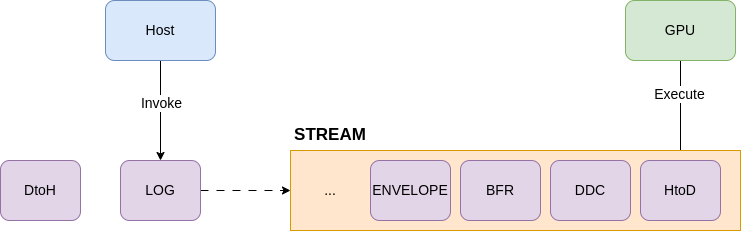
\includegraphics[scale=0.4]{imgs/stream_queue.png}
  \end{figure}  

\end{frame}


\begin{frame}[fragile]{CUDA Streams: example}


\begin{lstlisting}
  rf_gpu.set(rf_cpu)   # HtoD
  iq = ddc_kernel(rf_gpu) # DDC
  hri = delay_and_sum_kernel(iq)  # BFR
  envelope = envelope_kernel(hri)  # ENVELOPE
  bmode = log_compression_kernel(envelope) # LOG
  bmode_cpu = bmode.get() # DtoH
\end{lstlisting}


  \begin{figure}
    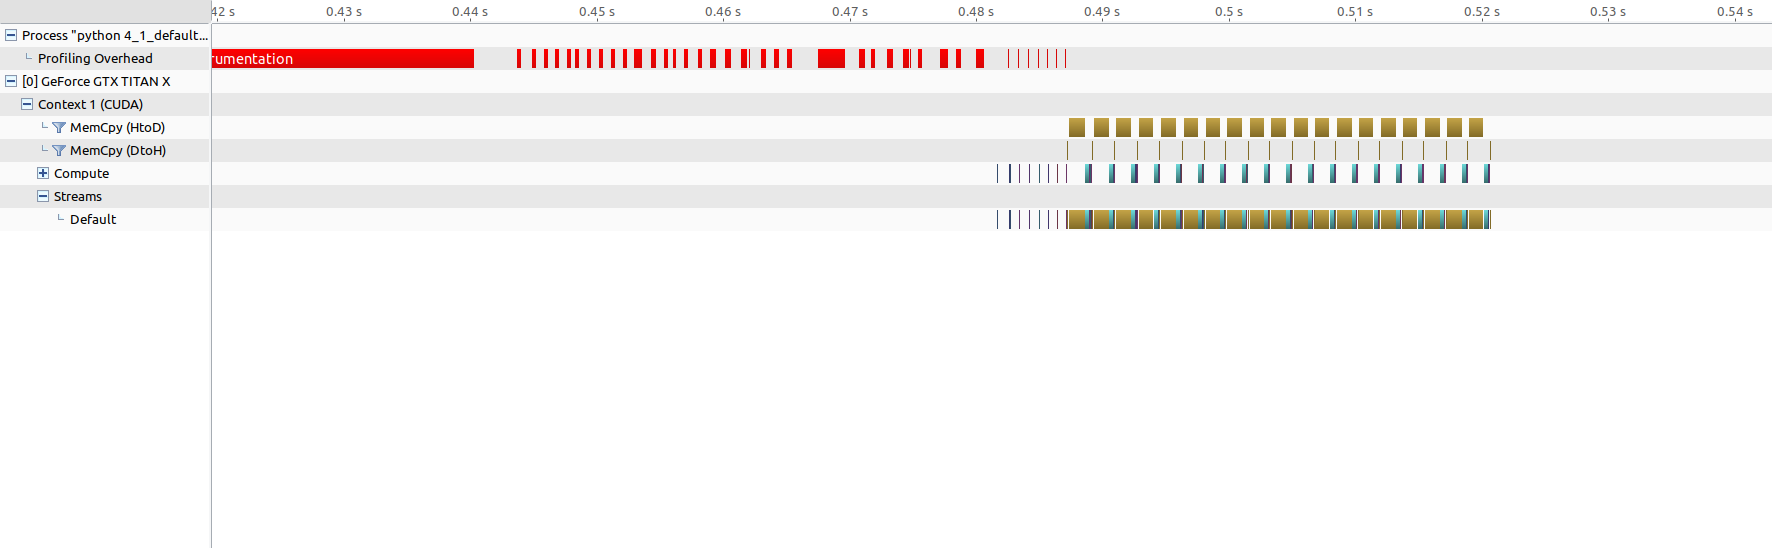
\includegraphics[scale=0.2]{imgs/single_stream.png}
  \end{figure}  

\end{frame}



\begin{frame}{CUDA Streams: multiple streams}
  Is it possible to run GPU operations in parallel?
  \begin{itemize}
    \item Generally, it's possible, by using multiple streams.
    \item In practice: it depends what operations we would like to run in parallel:
      \begin{itemize}
        \item executing GPU kernels simultaneously -- not always guaranteed (it depends on the GPU occupancy, kernel scheduler implementation, etc.)
        \item GPU kernels and data transfers can be overlapped -- data transfers can be handled by a separate GPU component \textbf{DMA}, that can run in parallel with SMs
      \end{itemize}
  \end{itemize}
\end{frame}

\begin{frame}[fragile]{CUDA Streams: overlapping data transfer with kernels}

  \begin{lstlisting}
  stream_17 = cp.cuda.Stream(non_blocking=True)
  stream_18 = cp.cuda.Stream(non_blocking=True) 
  with stream_17:
    gpu_array.set(rf)
    img      = beamformer.process(gpu_array)
    envelope = to_envelope.process(img)
    bmode    = to_bmode.process(envelope)
  with stream_18:
    a+b
  \end{lstlisting}

  \begin{figure}
    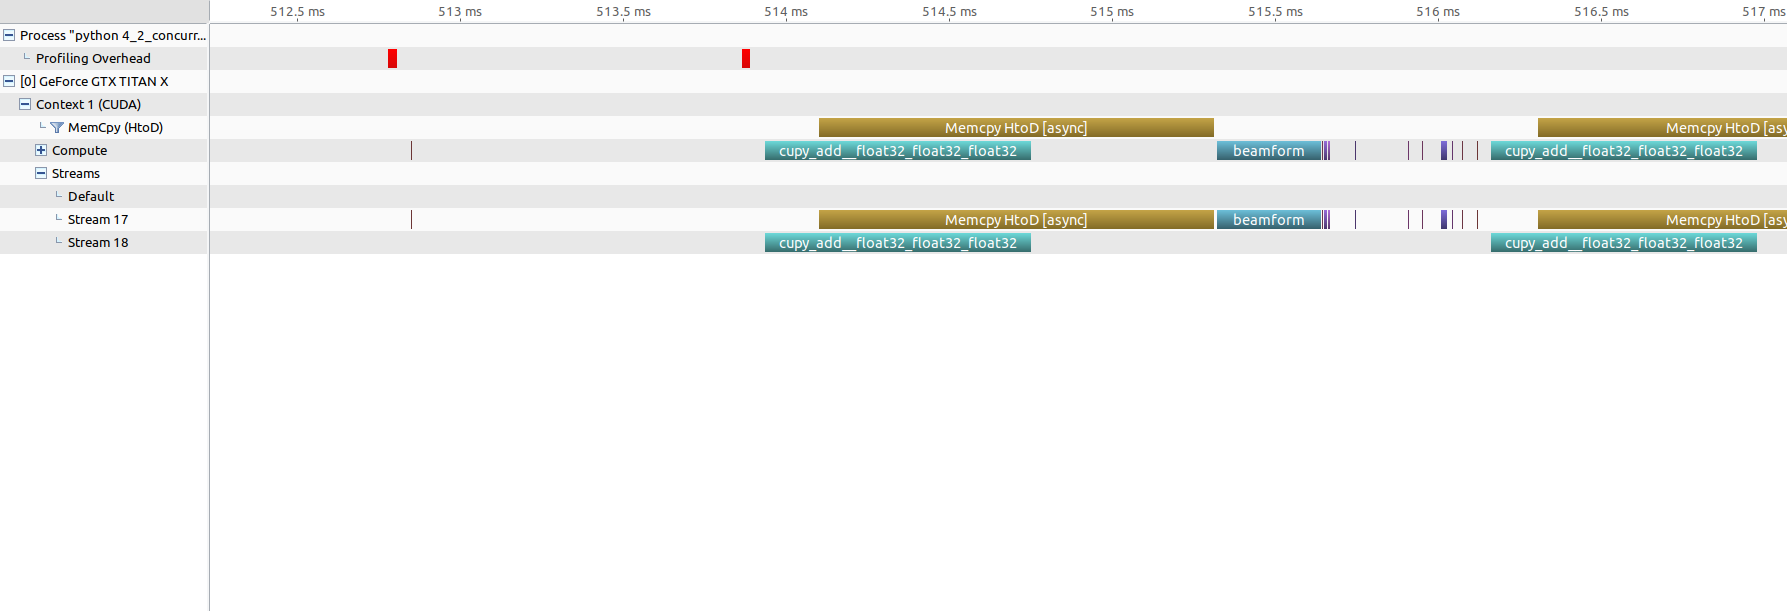
\includegraphics[scale=0.2]{imgs/concurrent_streams.png}
  \end{figure}  
\end{frame}

\begin{frame}{CUDA Streams synchronization: Events}

  How to make sure, that GPU kernel will not start until the HtoD transfer is finished?
  \begin{itemize}
    \item We can use CUDA \textbf{Events}.
    \item \textbf{CUDA event} object represents an event in the CUDA stream execution timeline. An example of such an event is the completion of a GPU kernel, or that the data transfer from host to GPU has finished.
  \end{itemize}

\end{frame}

\begin{frame}[fragile]{CUDA Streams synchronization: Events}

\begin{lstlisting}
    data_is_ready = cp.cuda.Event()
    gpu_array.set(rf, stream=HtoD_Stream) 
    data_is_ready.record(stream=HtoD_Stream) 
    processing_stream.wait_event(data_is_ready) 
    with processing_stream:
      some_processing(gpu_array)
\end{lstlisting}


  \begin{figure}
    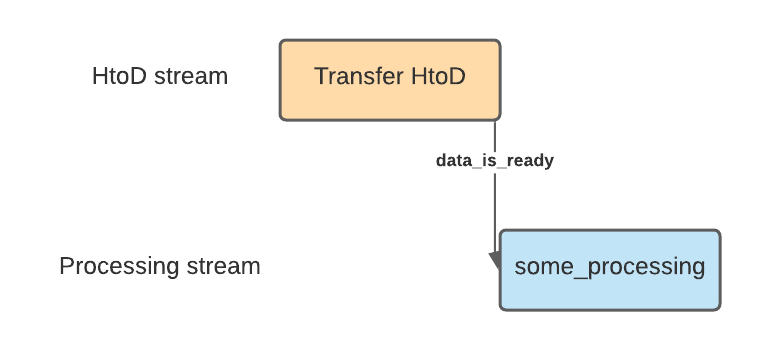
\includegraphics[scale=0.8]{imgs/events.png}
  \end{figure}  

\end{frame}


\begin{frame}[fragile]{CUDA Streams synchronization: Events}

  \begin{lstlisting}
    data_is_ready = cp.cuda.Event()
    gpu_array.set(rf, stream=HtoD_Stream) 
    data_is_ready.record(stream=HtoD_Stream) 
    processing_stream.wait_event(data_is_ready) 
    with processing_stream:
      some_processing(gpu_array)
  \end{lstlisting}


  \begin{figure}
    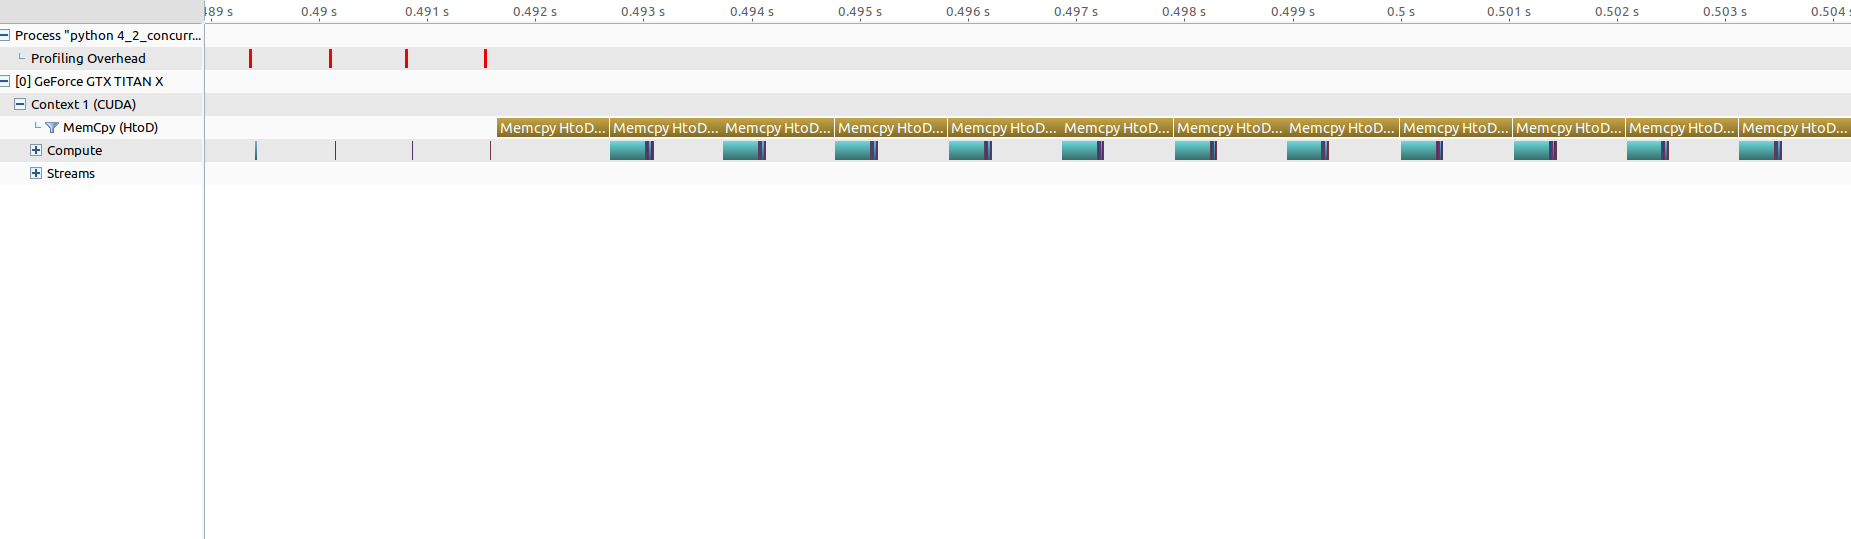
\includegraphics[scale=0.2]{imgs/concurrent_streams_sync.png}
  \end{figure}  

\end{frame}


\begin{frame}{Graph o operations}

  It's possible to use CUDA kernels and events to implement a graph of operations.

  Graph of operations: a Graph $G(V, E)$, where:
  \begin{itemize}
    \item $V$: \textbf{operations}
    \item $E$: \textbf{dependencies} between operations (input/output arrays)
  \end{itemize}

\end{frame}

\begin{frame}{Graph o operations: example}

  \begin{figure}
    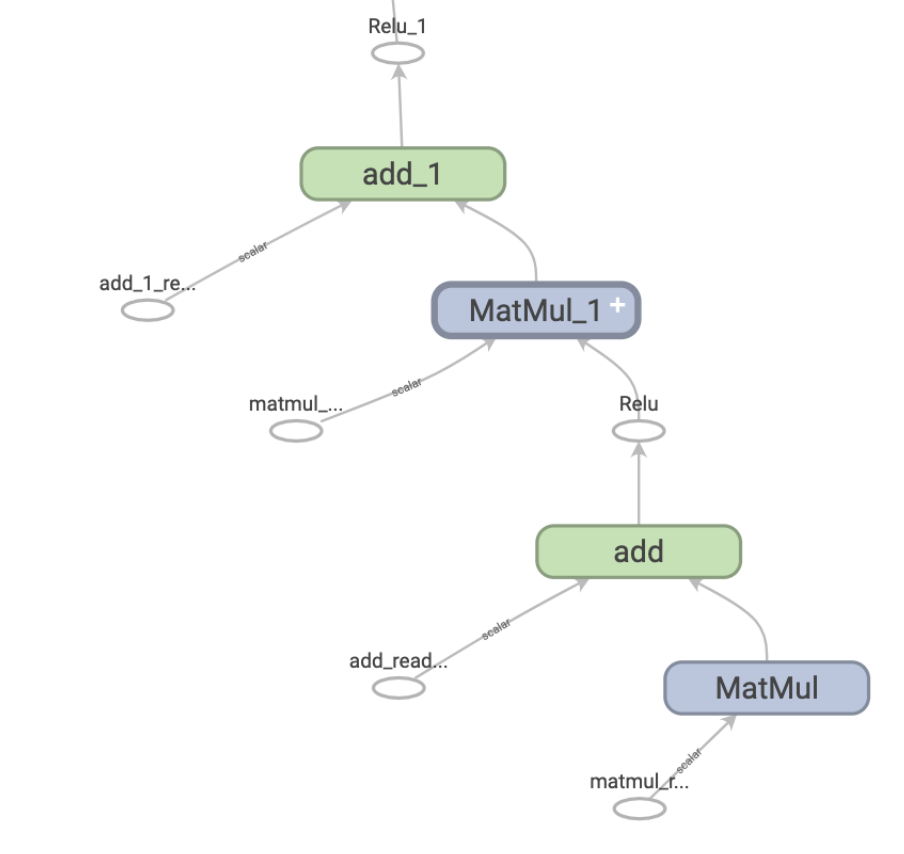
\includegraphics[scale=0.2]{imgs/tf_graph.png}
  \end{figure}
  \footnotesize Source: ''Tensorflow: introduction to graphs, \url{https://www.tensorflow.org/guide/intro_to_graphs}''
\end{frame}


\begin{frame}{Graph of operations: frameworks}

  \begin{itemize}
  \item tensorflow (based on XLA)
  \item ...
  \item NVIDIA CUDA Graphs
  \item NVIDIA CUDA Holoscan SDK
  \end{itemize}

\end{frame}

\begin{frame}{CUDA Graphs}
  \begin{figure}
    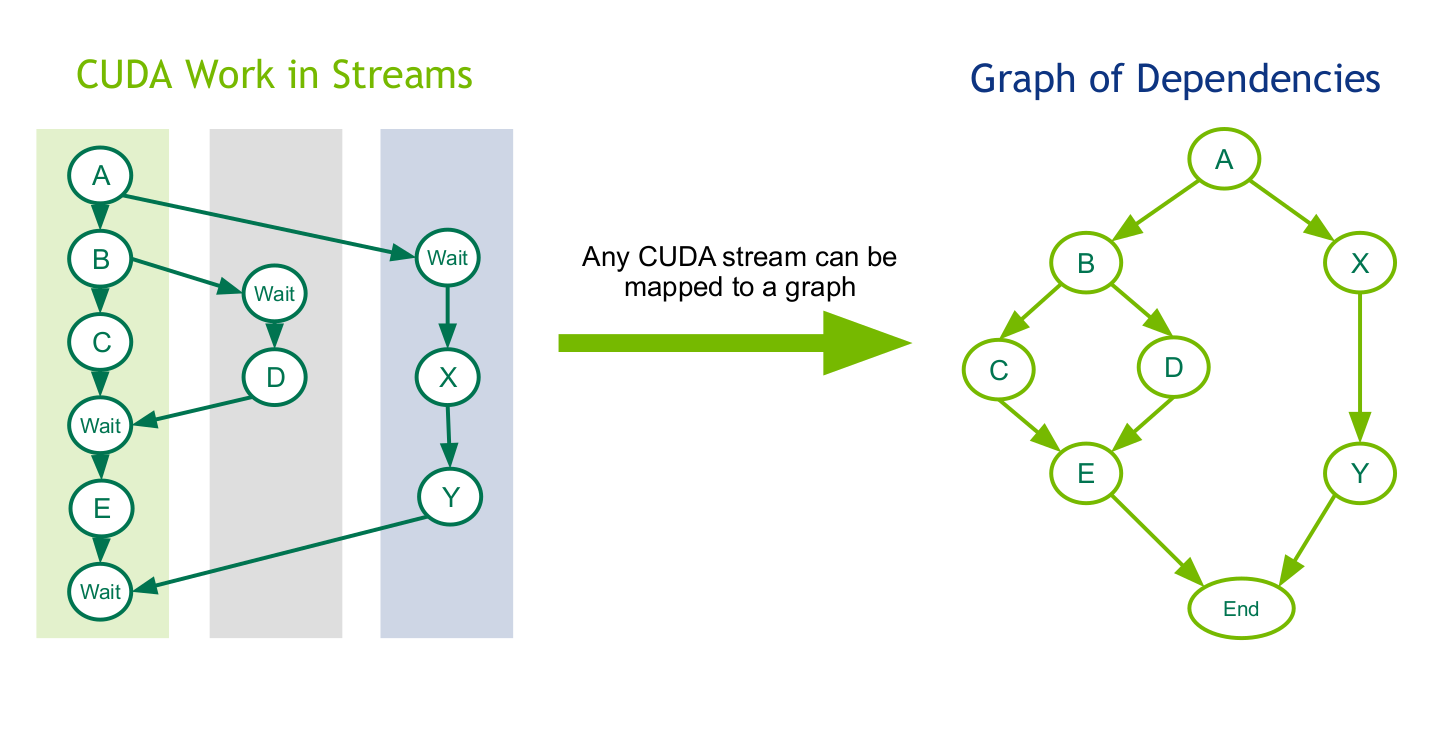
\includegraphics[scale=0.2]{imgs/cuda_graphs_streams_and_graphs.png}
  \end{figure}
  \footnotesize Source: ''013 NVIDIA CUDA Graphs'', \url{https://www.olcf.ornl.gov/wp-content/uploads/2021/10/013_CUDA_Graphs.pdf}
\end{frame}

\begin{frame}{CUDA Graphs: Execution model}
  \begin{figure}
    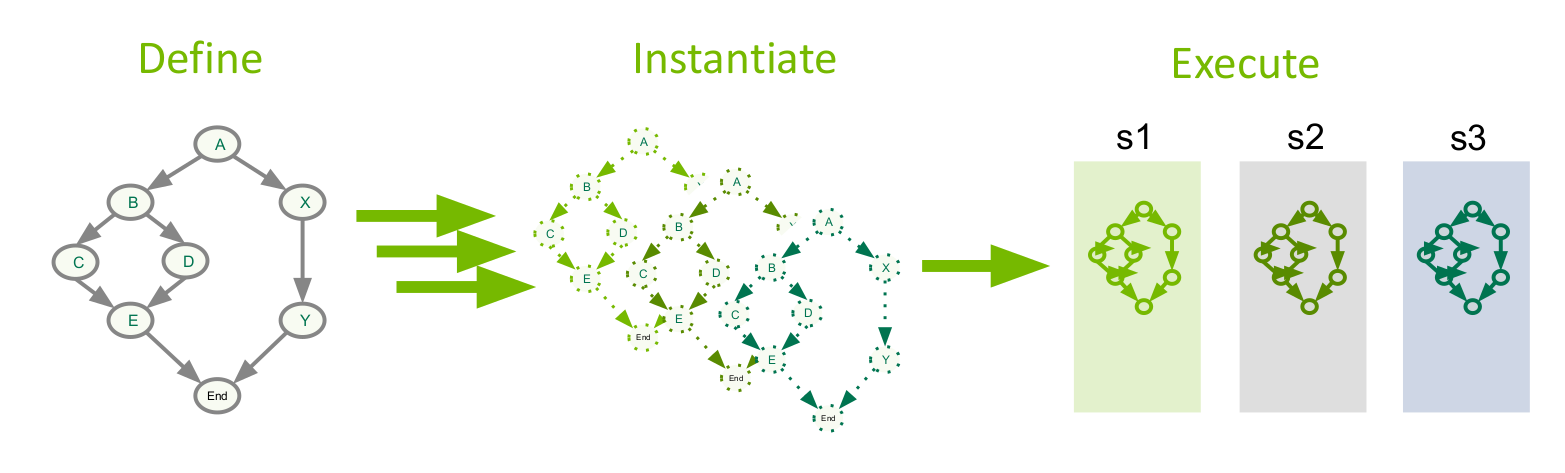
\includegraphics[scale=0.2]{imgs/cuda_graphs_execution_model.png}
  \end{figure}
\end{frame}

\begin{frame}{CUDA Graphs: kernel invocation overhead reduction}
  \begin{figure}
    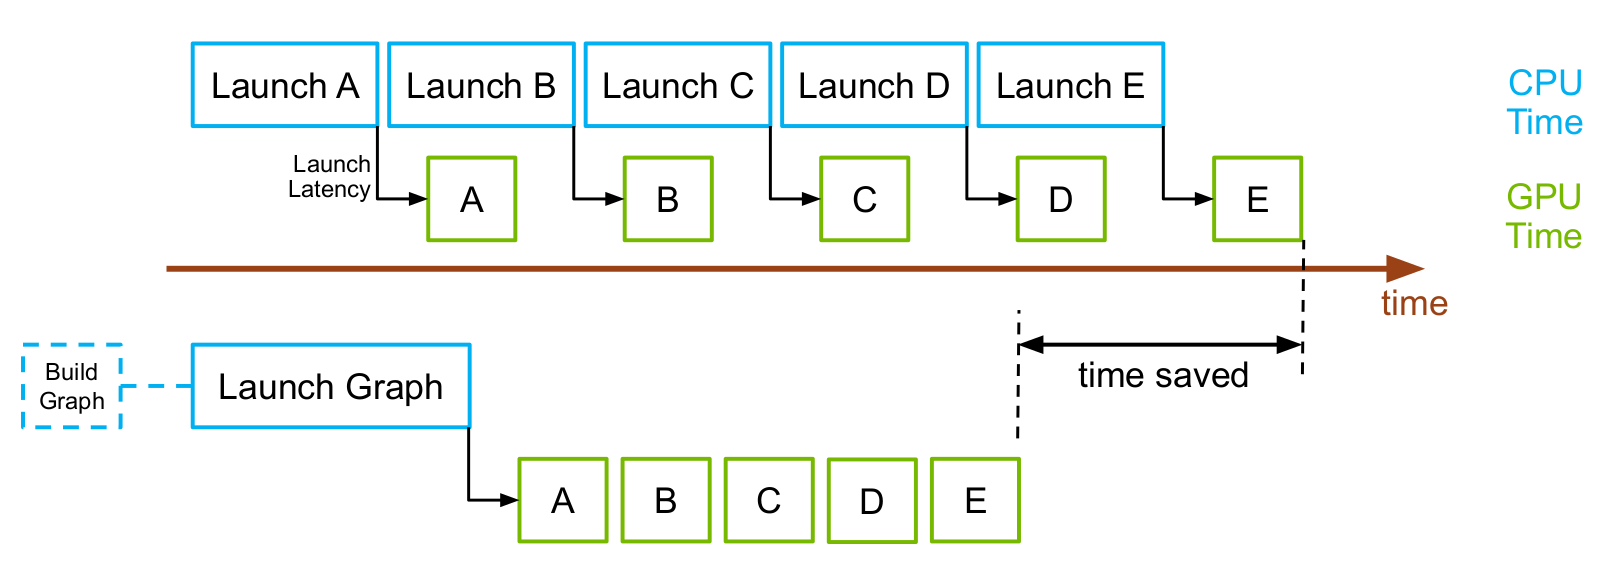
\includegraphics[scale=0.2]{imgs/cuda_graphs_kernel_invocation_overhead_reduction.png}
  \end{figure}
  \footnotesize Source: ''013 NVIDIA CUDA Graphs'', \url{https://www.olcf.ornl.gov/wp-content/uploads/2021/10/013_CUDA_Graphs.pdf}
\end{frame}


\begin{frame}{NVIDIA Holoscan SDK}
  \textbf{NVIDIA Holoscan} is the AI sensor processing platform that combines:
  \begin{itemize}
  \item hardware systems for low-latency sensor and
  \item network connectivity,
  \item optimized libraries for data processing and AI,
  \item ...
  \end{itemize}  

  \textbf{NVIDIA Holoscan SDK} is a development kit that provides:
  \begin{itemize}
  \item C++ and Python API,
  \item Built-in, common operators (AI inference, etc.),
  \item examples, a remote reopsitory of operators, performance tools...  
  \end{itemize}  

  \footnotesize Source: ''013 NVIDIA CUDA Graphs'', \url{https://www.olcf.ornl.gov/wp-content/uploads/2021/10/013_CUDA_Graphs.pdf}
\end{frame}


\begin{frame}{NVIDIA Holoscan SDK: Core concepts}

  Holoscan SDK implements a custom graph framework: \textbf{Graph Execution
    Framework (GXF)}.

  Also provides a native support for:
  \begin{itemize}
  \item GPU Direct RDMA
  \item TensorRT
  \item ...  
  \end{itemize}  
  
\end{frame}

\begin{frame}{NVIDIA Holoscan SDK: Core concepts}
  An \textbf{Application} is composed of \textbf{Fragments}, each of which runs
  a sub-graph of \textbf{Operations}.

  \begin{figure}
    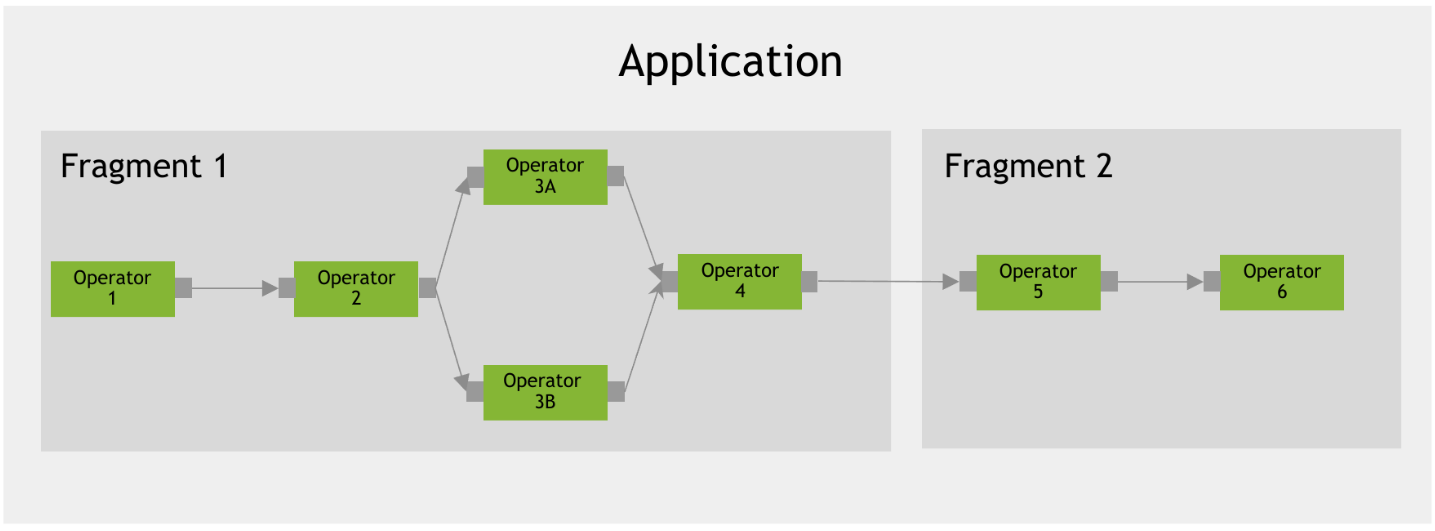
\includegraphics[scale=0.2]{imgs/holoscan_application.png}
  \end{figure}
  
\end{frame}

\begin{frame}{NVIDIA Holoscan SDK: Core concepts}
  \textbf{Operator} is a basic unit of work. An operator receives streaming data
  at an input port, processes it, and publishes it to one of the output ports.

  \begin{figure}
    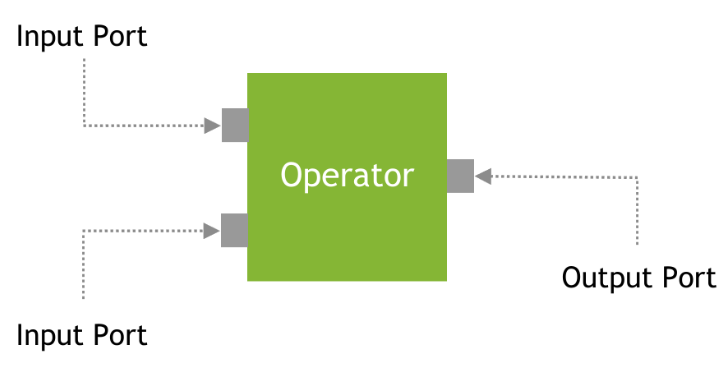
\includegraphics[scale=0.2]{imgs/holoscan_operator.png}
  \end{figure}
  
\end{frame}


\begin{frame}{NVIDIA Holoscan SDK}
  HoloHub: a central repository to share reusable operators and applications with the Holoscan community.
  
  In preparation:
  \begin{itemize}
    \item us4us us4R ←→ NVIDIA Holoscan SDK integration
    \item GPU RCA image reconstruction using NVIDIA Holoscan SDK (offline processing)
    \end{itemize}

    Please make sure to subscribe to the `github.com/lab4us/gpu-short-course`
    repository by pressing 'Star' button. This way you will get notification
    when the above are ready. Thanks!

\end{frame}

\end{document}
